\documentclass[12pt]{beamer}
\usetheme{Berlin}
\usepackage[utf8]{inputenc}
\usepackage{amsmath}
\usepackage{amsfonts}
\usepackage{amssymb}
\usepackage{graphicx}
\usepackage{subfigure}
\usepackage{caption}
\usepackage{multicol}
\usepackage[spanish,es-tabla]{babel}
\usepackage{multirow}
\usepackage[T1]{fontenc}
\usepackage{mathptmx}
\usepackage{multicol}
\usepackage{float}
\author{Métodos númericos.}
\title{Métodos: Splines, Simpson, Runge-Kutta}
%\setbeamercovered{transparent} 
\setbeamertemplate{navigation symbols}{} 
%\logo{} 
\institute{Facultad de Ciencias Físico Matemáticas, UAdeC.} 
\date{4 de diciembre de 2019. } 
\subject{Métodos númericos.} 
\begin{document}

\begin{frame}
\titlepage
Gerardo de la Cruz Cantú. \\ Luis Eduardo Sánchez González.
\end{frame}

\begin{frame}
\tableofcontents
\end{frame}

\section{Método de Splines.}
\subsection{Trazadores cúbicos.}
\begin{frame}{¿Qué son los Splines?}
Aproximación polinómica fragmentaria.
\begin{figure}
\centering
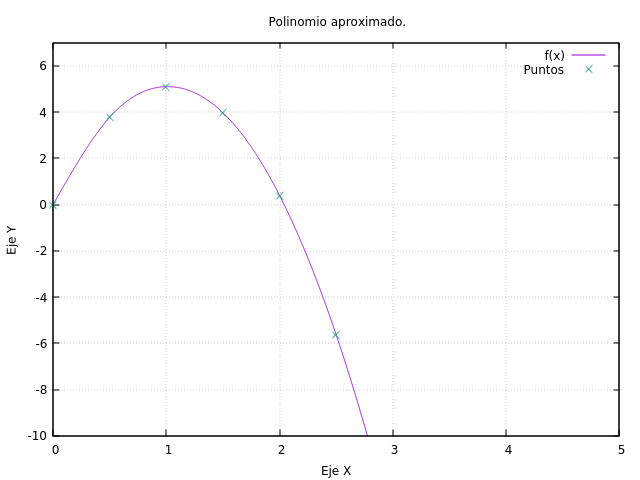
\includegraphics[scale=0.4]{spline.png}
\caption{Función aproximada por medio de Splines cúbicos.} 
\end{figure}
\end{frame}

\begin{frame}{¿Por qué los trazadores cúbicos son mejor aproximación?}
\begin{figure}[H]
\centering
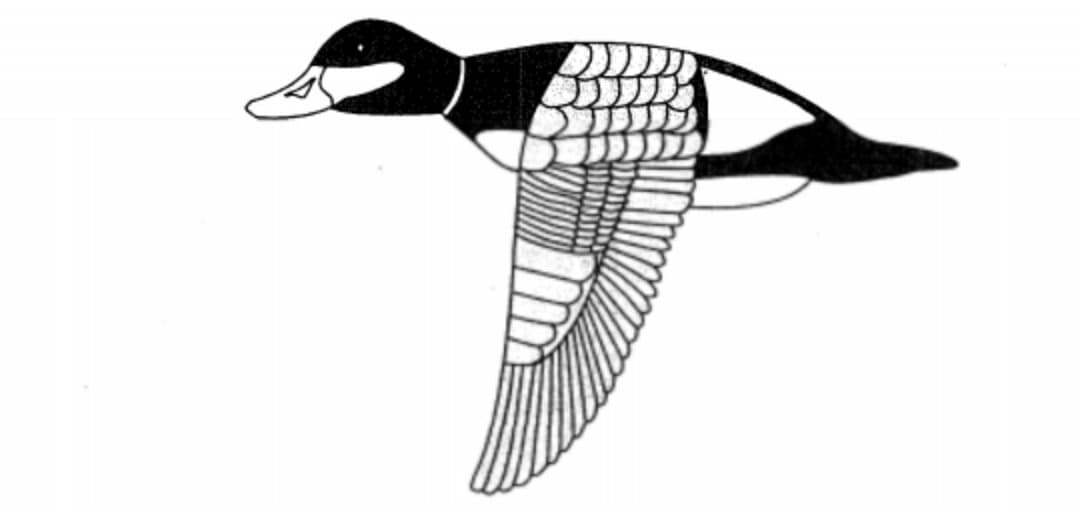
\includegraphics[scale=0.15]{77353545_2546339105577443_6082688536073469952_n.jpg} 
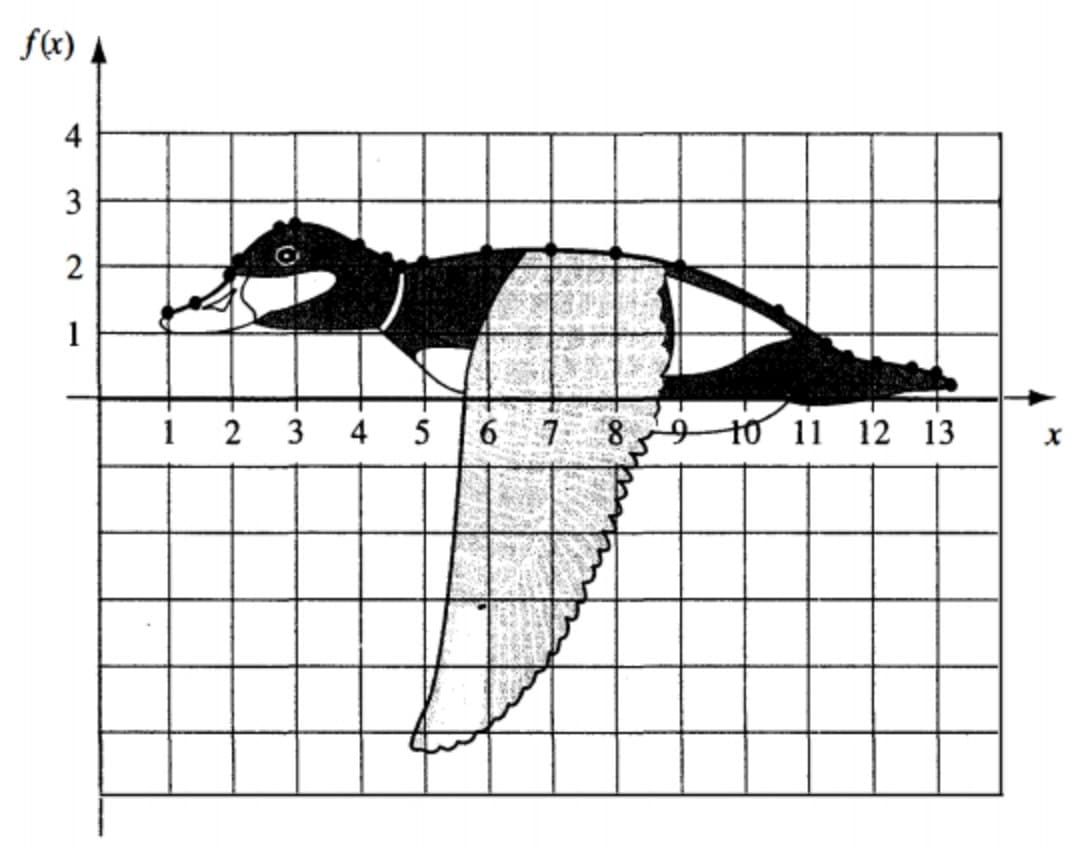
\includegraphics[scale=0.15]{74614877_953192571727341_6632384722930499584_n.jpg} 
\end{figure}
\end{frame}

\begin{frame}{Comparación de Splines con Interpolación simple.}

\begin{figure}[H]
\centering
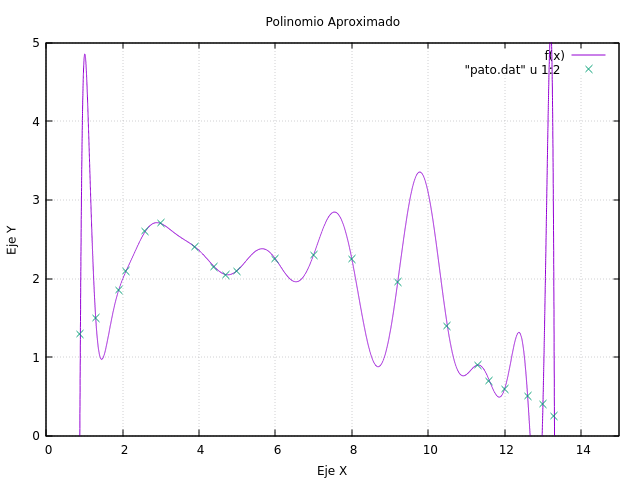
\includegraphics[scale=0.3]{patointer.png} 
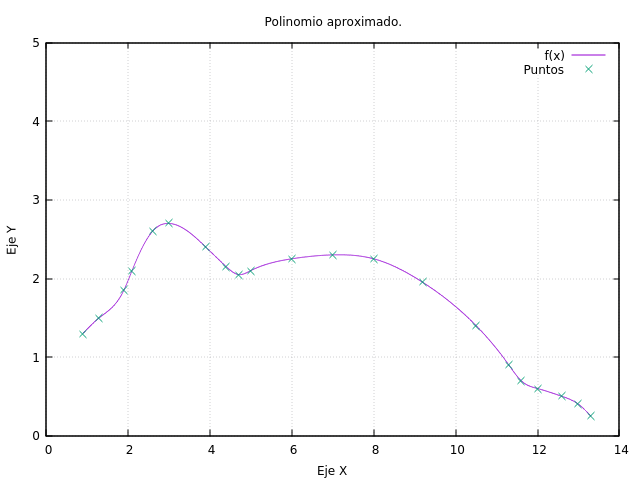
\includegraphics[scale=0.3]{graficapatosplines.png} 
\caption{Gráfica de pato que vuela, interpolación simple vs interpolación splines}
\end{figure}

\end{frame}
\subsection{Movimiento de una pelota en caida libre.}
\begin{frame}{Problematica: Estimar la función de la posición de una pelota que cae.}
Cuando se lanza una pelota al aire se van obteniendo los datos de la posición de la pelota en ciertos intervalos de tiempo, se tiene la siguiente tabla. Se desea aproximar una función a estos datos de manera que sea lo más exacto posible.
\begin{table}[H]
\centering
\begin{tabular}{|c|c|} \hline
t(s) & $\Delta $ y(m) \\ \hline 
0 & 0 \\ \hline 
0.5 & 3.7737 \\  \hline 
1.5 & 5.095 \\ \hline 
2 & 3.9637 \\ \hline 
2.5  & 0.38 \\ \hline 
\end{tabular} 
\end{table}
\end{frame}


\section{Método de Simspon.}
\subsection{Integración númerica.}
\begin{frame}{Integración numérica.}

Método de Simpson $\frac{1}{3}$.
\begin{equation}
\int _{x_{0}} ^{x_{2}} f(x) dx =  \dfrac{h}{3}[f(x_{0}) + 4f(x_{1}) + f(x_{2})]
\end{equation}

Método de Simpson $ \frac{3}{8}$.
\begin{equation}
\int_{x_{0}} ^{x_{3}} f(x) dx = \dfrac{3h}{8}[f(x_{0}) + 3f(x_{1}) + 3f(x_{2}) + f(x_{})]
\end{equation}

\end{frame}
\begin{frame}
\begin{figure}[H]
\centering
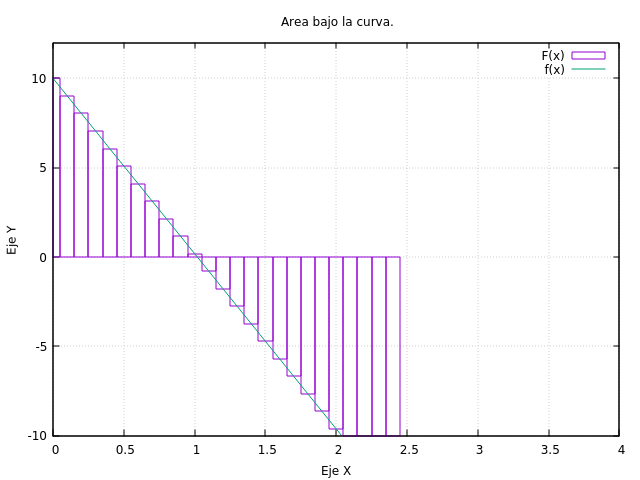
\includegraphics[scale=0.5]{simpson.png} 
\caption{Área bajo la curva de una función f(x)}
\end{figure}
\end{frame}


\subsection{La pelota que cae.}
\begin{frame}{Problematica: La pelota que cae.}
Un niño lanza una pelota al aire con una velocidad Vo, se sabe que la velocidad de la pelota estará dada por la siguiente ecuación:
$$ V(t) = Vo - gt $$
donde $Vo$ es la velocidad inicial con la que sale la pelota, $g$ es el valor de gravedad tal que $ g =  9.81 \; \frac{m}{s^{2}} \; $ y $t$ es el tiempo medido en segundos. ¿Cuál es el desplazamiento de la pelota despues de $t = 2 s$?
\end{frame}


\section{Método de Runge-Kutta.}
\subsection{Resolución de ecuaciones diferenciales.}
\begin{frame}{Método de Runge-Kutta de cuarto orden.}
Método de Runge-Kutta de orden cuatro.
$$ y_{0} = t_{0} $$
$$ K_{1} = hf(t_{i}, y_{i})$$
$$ K_{2} = hf(t_{i} + \frac{h}{2}, y_{i} + \frac{1}{2} K_{1})$$
\end{frame}
\begin{frame}{Método de Runge-Kutta de cuarto orden.}
$$ K_{3} = hf(t_{i} + \frac{h}{2}, y_{i} + \frac{1}{2} K_{2})$$
$$ K_{4} = hf(t_{i+1}, y_{i} + K_{3})$$
$$ y_{i+1} = y_{i} + \frac{1}{6}(K_{1} + 2K_{2} + 2K_{3} + K_{4})$$
\end{frame}
\subsection{Pelota como proyectil.}
\begin{frame}{Problematica: Trayectoria de un proyectil.}
Después de un largo rato jugando con la pelota el niño decide lanzar la pelota con un cierto ángulo $\theta$ de inclinación a una velocidad $Vo$, la pelota sale disparada y su trayectoria puede modelar con la siguiente ecuación diferencial.
$$ r'(t) = \langle VoCos( \theta ), VoSen( \theta ) - gt \rangle $$
Encontrar la solución númerica a este problema.
\end{frame}

\end{document}